\chapter{Executive Overview}
\label{ch:Executive_Overview}
This report aims to present an innovative design for an Inter-Urban Air Mobility (UAM) vehicle, poised to transform short-to-medium distance transportation.
The design focuses on an electric Vertical Take-Off and Landing (eVTOL) vehicle intended for travel within and between urban areas.
A key challenge in Urban Mobility is addressing the last-mile issue; creating a vehicle with a minimal ground footprint that requires less landing space. Therefore, it can land at vertiports in very densely populated areas.
Additionally, recognising the imminent environmental challenges, the project prioritises minimising the vehicle's environmental impact.

The Mission Need Statement (MNS) and Project Objective Statement (POS) are as follows:

\paragraph{MNS:}“\textit{Achieve Sustainable Inter-Urban Air Mobility with a low ground footprint vehicle.}”
\vspace{-5mm}
\paragraph{POS:}“\textit{Design a low ground footprint, sustainable, urban transwing electric Vertical Take-Off and Landing vehicle within production costs of \qty{2}{M\texteuro}, by ten students in ten weeks time.}”


\section*{The Concept}
The chosen concept has rotating wings, so the aircraft has two configurations. The first configuration is in cruise, where the wings are fully unfolded, and the \textit{Swing eVTOL} flies like a general aviation aircraft. The second configuration is in hover, where it flies as a rotorcraft. The \textit{Swing eVTOL} will take off in hover configuration, transition mid-air to cruise configuration to fly further and transition back to hover configuration to land. The rotating wings allow for very efficient cruise and a low ground footprint for landing.

\section*{Market Analysis}
To analyse the rapidly expanding Urban Air Mobility (UAM) market, market segmentation is defined, and competitors are analysed. The current market segments are air taxis,  airport shuttles, and interurban transport. Due to the low ground footprint and high range, the \textit{Swing eVTOL} can be used in any of these markets and differentiates itself by also providing last-mile transport.
Moreover, the Competition Analysis found that the main competitors are the Joby S4 and Archer Midnight, which both lack the low ground footprint and range combination, which provides the solution to the last-mile problem, establishing the \textit{Swing's} differentiation factor as can be seen in \Cref{tab_exe:possible_usecases}. 

\begin{table}[H]
    \centering
    \caption{Differentiation of \textit{Swing eVTOL} in market segments}
    \label{tab_exe:possible_usecases}
    \resizebox{0.8\textwidth}{!}{%
    \begin{tabular}{l|c|c|c|c}
        \toprule
        \textbf{eVTOL}       & \textbf{Air Taxi }    &  \textbf{Airport Shuttle} &\textbf{Intercity Flights}    &   \textbf{Last-mile transport}     \\ \midrule
        \textit{Swing}        &X& X & X & X             \\
        Joby S4    &X& X & X & -             \\
        Archer Midnight   &X& X & - & -             \\
        EHang 216-S    &X& - & - & X             \\\bottomrule
    \end{tabular}%
    }
\end{table}
Furthermore, London is found to be the ideal geographical location linked to the four possible segments, and it provides the perfect partner in the UK Air Mobility Consortium. The Consortium will provide the perfect environment for UAM implementation, testing, and regulations.


\section*{Technical Risk Analysis}
% \todo[inline]{rewrite this, to also include hinge failure, engine failure and battery failure}
The technical risk analysis is a critical part of the project, as it identifies the likelihood and impact of potential risks associated with the \textit{Swing's} design and development.
Key risks include propulsion failure, structural integrity of the aircraft and hinge, and power system reliability.
Then, mitigation strategies and contingency plans are outlined for each identified risk, ensuring the project can navigate technical challenges effectively.
Examples of mitigation strategies are extensive testing and timely maintenance, and examples of contingency plans are detailed emergency procedures and protocols and emergency landing procedures.
The successful integration was established through the improved risk maps.


\section*{Mission Profile}
The mission profile for the \textit{Swing eVTOL} is meticulously designed to ensure optimal performance and energy efficiency.
The profile is divided into two main parts: the normal operational range and the emergency deviations.
To ensure a longer battery life, only 60 \% of the battery is used, but for emergencies, this full battery could be used.
The mission profile starts with a vertical climb, followed by a transition to cruise configuration and a climb to cruise altitude.
After cruise, the \textit{Swing eVTOL} will descend and transition to hover configuration,
so it can land vertically.
The altitude and power of the aircraft for a typical mission of \qty{250}{km} can be seen in \Cref{fig_exe:mission_profile}.

\begin{figure}[!hptb]
    \centering
    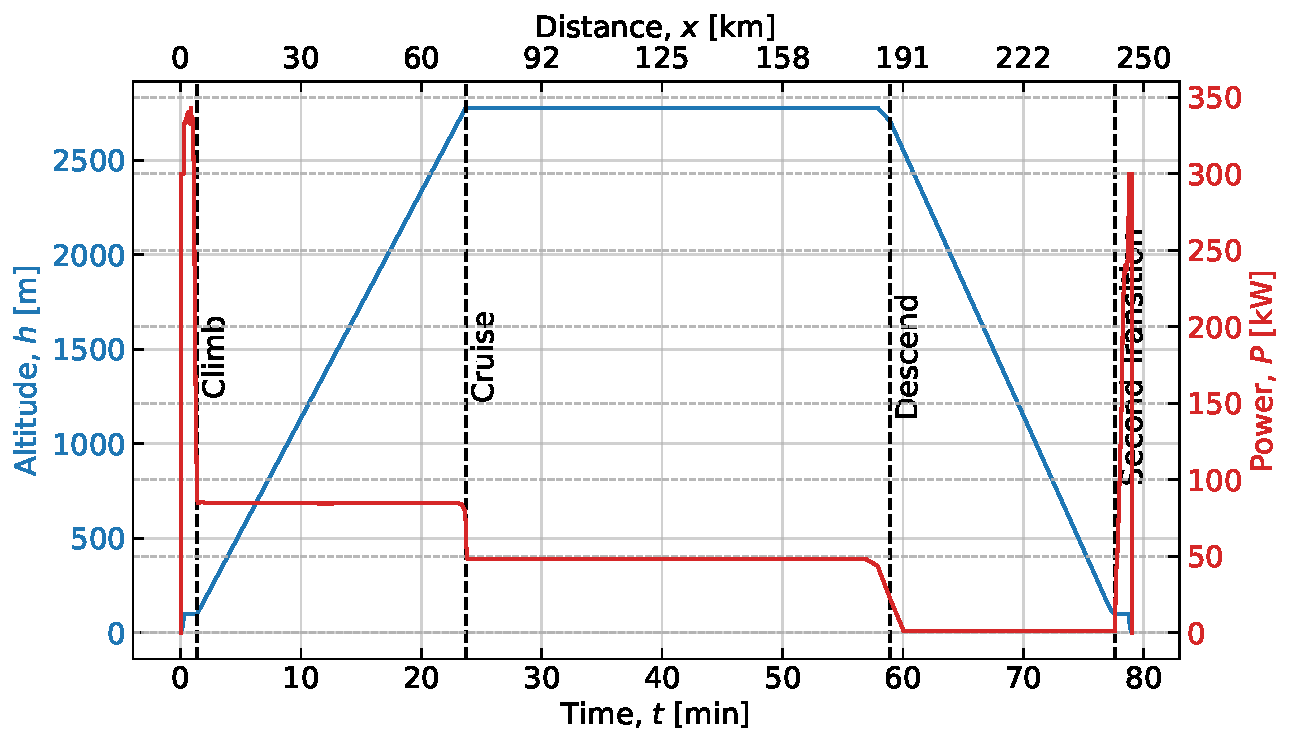
\includegraphics[height=0.3\textheight]{figures/MissionProfile/mission_profile_over_time_and_distance_max_range}
    \caption{Altitude and engine power over distance and time of the mission profile with maximum range}
    \label{fig_exe:mission_profile}
\end{figure}

The mission profile is optimised to minimise the aircraft’s total energy consumption.
This is achieved through a multiphase optimisation approach, where the different mission phases are modelled and optimised separately.
The optimisation process considers various factors, such as the power required, the thrust produced by the engines, and the aerodynamic forces acting on the aircraft.
The energy distribution resulting from the optimisation can be seen in \Cref{fig_exe:energy_distribution}.

\begin{figure}[H]
    \begin{subfigure}[b]{0.49\textwidth}
        \centering
        
\includegraphics[width=0.9\linewidth]{figures/MissionProfile/energy_distribution}
        \caption{Energy distribution of the nominal mission profile}
        \label{fig_exe:nominal_energy_distribution}
    \end{subfigure}
    \hfill
    \begin{subfigure}[b]{0.49\textwidth}
        \centering
        
\includegraphics[width=0.9\linewidth]{figures/MissionProfile/energy_distribution_max_range}
        \caption{Energy distribution of the mission profile with maximum range}
        \label{fig_exe:energy_distribution_max_range}
    \end{subfigure}
    \caption{Energy distribution over the different phases of the mission profiles}
    \label{fig_exe:energy_distribution}
\end{figure}

\section*{Detailed Subsystem Design}
Now that the mission profile is known, it is possible to start looking into the detailed design. The detailed design phase can be divided into six main subsystems that shape the \textit{Swing eVTOL}.

\subsection*{\textit{Aerodynamics}} 
The first subsystem that was designed is the Aerodynamics subsystem.
From class I and class II estimations, a wing area of 14m is found,
the wing planform was then optimised for the ground footprint, and the final wing parameters can be found in \Cref{tab:exewing_planform}.
From the airfoil analysis, the Eppler 560 airfoil was considered to be the best fit for the \textit{Swing eVTOL}.
After in-depth ergonomic analysis,
it was found that the outer fuselage diameter is \qty{1.7}{m}
and that the fuselage should have a tadpole shape with a length of \qty{8}{m}.

\begin{table}[ht]
  \hspace{-0.75cm}
  \begin{minipage}{0.75\textwidth}
    \centering
    
\includegraphics[width=1\linewidth]{figures/AerodynamicAnalysis/rotating_wing_three_view}
    \captionof{figure}{Parametric Model used for Aerodynamic analysis}
    \label{fig:exeParametric}
  \end{minipage}
  \begin{minipage}{0.2\textwidth}
    \centering
    \caption{Aerodynamic design values}
    \label{tab:exewing_planform}
    \begin{tabular}{
        @{}
        >{$}l<{$}
        |S[table-format=2.2]
        >{\collectcell\unit}l<{\endcollectcell}
        @{}
    }   
        \toprule
        S                 & 14            &  m^2        \\
        b                 & 14            &  m          \\
        A                 & 14            &  -          \\
        c_\text{r}        & 1.42          &  m          \\
        c_\text{t}        & 0.57          &  m          \\
        \mathrm{MAC}      & 1.06          &  m          \\
        y_\mathrm{MAC}    & 3.0           &  m          \\
        \Lambda_{c/4}     & 0             &  deg        \\
        \Lambda_{LE}      & 2             &  deg        \\
        \lambda           & 0.4           &  -          \\
        \Gamma            & 1             &  deg        \\
        \midrule
        l_\text{fuselage}      & 8             & m           \\
        d_\text{fuselage}      & 1.7           & m           \\
        \midrule
        C_{D_0}           & 20.6          &  $10^{-5}$        \\
        \bottomrule
    \end{tabular}
  \end{minipage}
\end{table}
Class II drag estimations from Raymer \cite{raymer1992aircraft} were used to find a $C_{D_0}$ of \qty{0.00206}{}
The entire aircraft was then put into the AeroSandbox tool \cite{aerosandbox} as a parametric model, and more in-depth aerodynamic analysis was done to find stability derivatives.
The parametric model can be seen in \Cref{fig:exeParametric}


\subsection*{\textit{Power and Propulsion}}
After the aerodynamics and the weight of the aircraft have been established, with the maximum propeller diameter and number of engines of six (three engines per wing) obtained from considerations on geometry and disk loading, it is possible to determine the power curve of the \textit{Swing} eVTOL. To obtain the power used by the engines as a function of horizontal airspeed, a power model encompassing characteristics of both helicopters and conventional aircraft is used. For
the transition, required power and a surplus of power to facilitate acceleration are considered. This makes the transition phase the most power-hungry of the whole mission; \Cref{fig_exe:pcurveNOoptimisation} is thus inserted in this overview.

\begin{table}[ht]
  \hspace{-0.75cm}
  \begin{minipage}{0.7\textwidth}
    \centering
    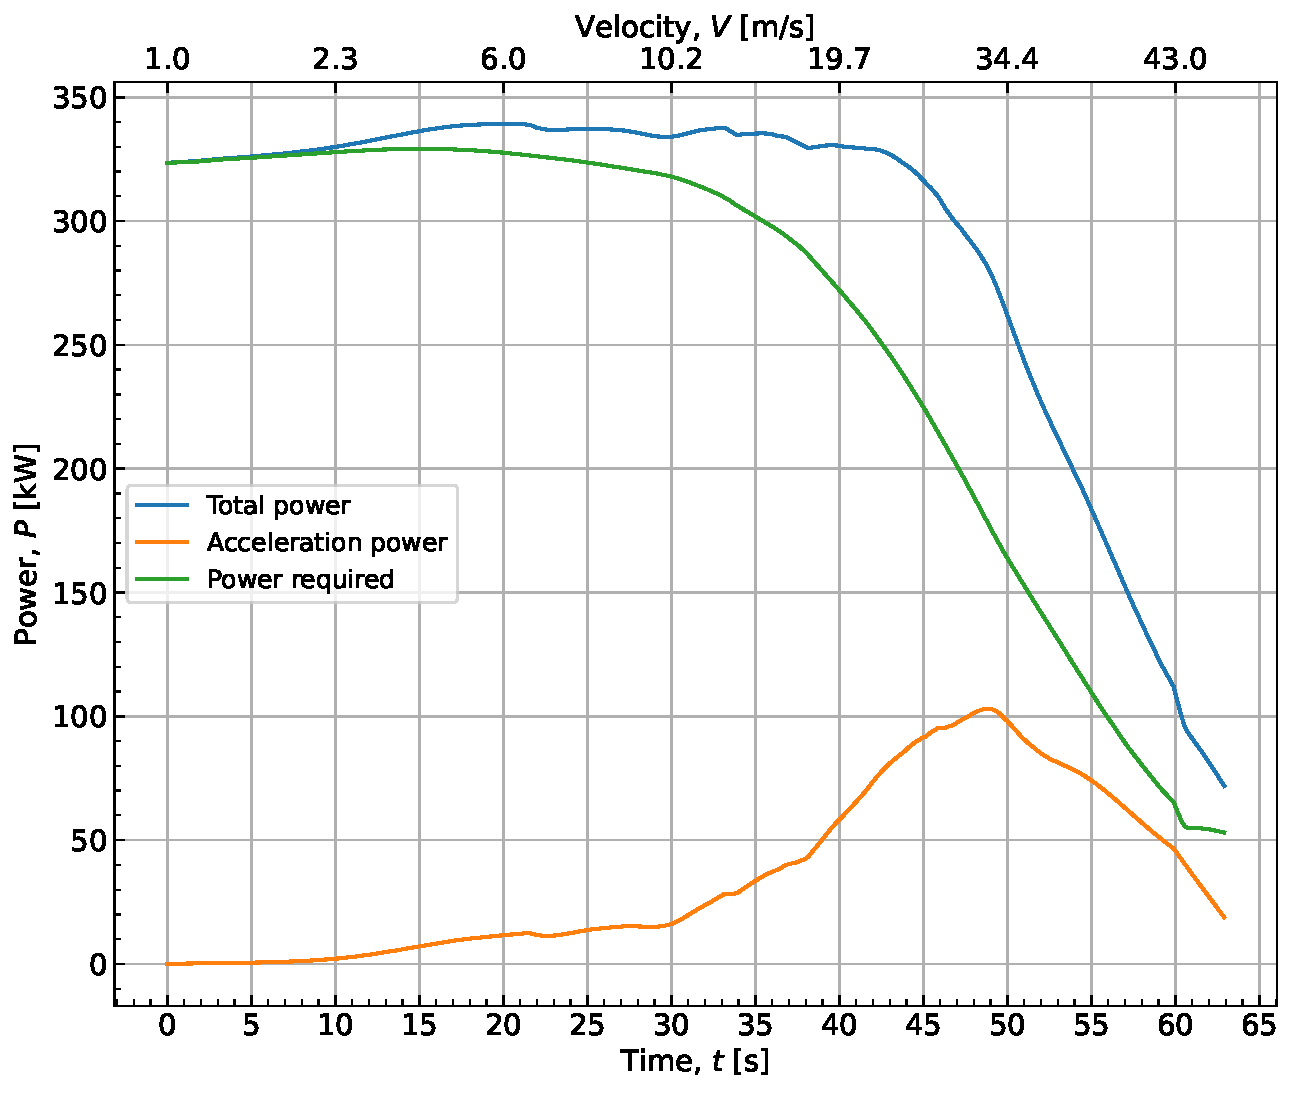
\includegraphics[width=0.8\linewidth]{figures/MissionProfile/power_over_velocity_and_time.pdf}
    \captionof{figure}{Power curve for the transition phase, where the highest power levels are experienced}
    \label{fig_exe:pcurveNOoptimisation}
  \end{minipage}
  \begin{minipage}{0.15\textwidth}
    \centering
    \caption{Specifications of the chosen motor}
    \label{tab_exe:motorspecs}
\begin{tabular}{|c|c|}
\hline
\textbf{Motor Name} & \textbf{Emrax 228} \\
\hline
$P_{\max}$ [kW] & 75 \\
\hline
$T_{\text{peak}}$ [Nm] & 130 \\
\hline
RPM$_{\max}$ (@$P_{\text{peak}}$) & 6500 (124) \\
\hline
Mass [kg] & 13.5 \\
\hline
$P/W$ [kW/kg] & 5.6 \\
\hline
$P_{\text{peak tot}}$ [kW] & 450 \\
\hline
$D \times L$ [mm] & 228 $\times$ 86 \\
\hline
\end{tabular}
  \end{minipage}
\end{table}

% \begin{figure}[htpb]
%     \centering
%     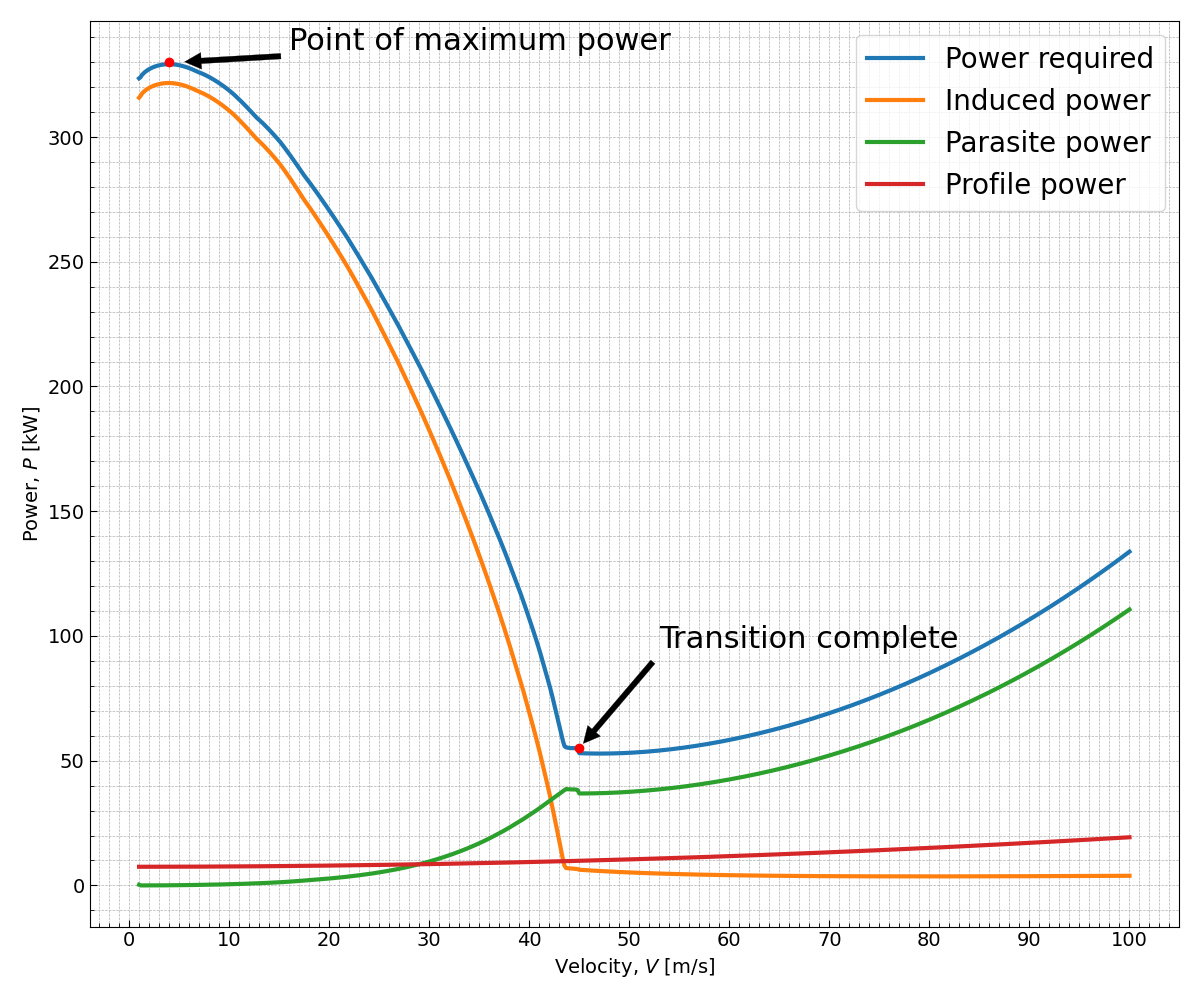
\includegraphics[width=0.7\linewidth]{figures/Propulsion/pcurveNONopt}
%     \caption{power required over velocity profile.}
%     \label{fig_exe:pcurveNOoptimisation}
% \end{figure}

Following the maximum total power of \qty{343}{kW}, along with the noise and thrust requirements, the propellers can be sized and the motor model selected. The specifications of the motor model chosen are tabulated in \Cref{tab_exe:motorspecs}, whereas the final design values of the propulsion system are found in \Cref{tab_exe:FinalPropValues}.
\begin{table}[H]
\caption{Final propeller parameters}
\label{tab_exe:FinalPropValues}
\centering
\begin{tabular}{cccccc}
    \toprule
$D_{\text{prop}}$ & Blade airfoil & Average blade chord &B & RPM      & $\beta$  \\\midrule
    \qty{2.1}{m}   & Clark-Y  & \qty{14.7}{cm}    & 6 & 500-1300 & $35\degree$  \\
    \bottomrule
\end{tabular}
\end{table}


\subsection*{\textit{Structures \& Materials}}
Given its great mechanical properties and weight savings, CFRP was chosen for most of the structure of the \textit{Swing}, except for wing structural components like spars and stiffeners, which are made of aluminium.
Glare is used for non-structural components on components most exposed to impacts due to its excellent tolerance to impact and damage.

The structural design focused on the design of the wing structure, as this was found to be the most structurally challenging component of the \textit{Swing} due to the lack of a pressurised fuselage.
A maximum load factor of 4.1 and a T/W ratio of 2 were used to compute the loads in cruise and vertical flight, respectively.
Wing spars were designed to take the bending moments as well as the torques.
The latter is also accounted for by the wing skin sizing, together with the buckling caused by compressive loads.
The rib locations are chosen strategically to introduce point forces caused by the engines, hinge, and control surfaces.
The final wing structural parameters are shown in \Cref{tab:finalwingstructure}, with their meaning indicated in \Cref{fig:wingboxexe}.

\begin{figure}[H]
    \centering
    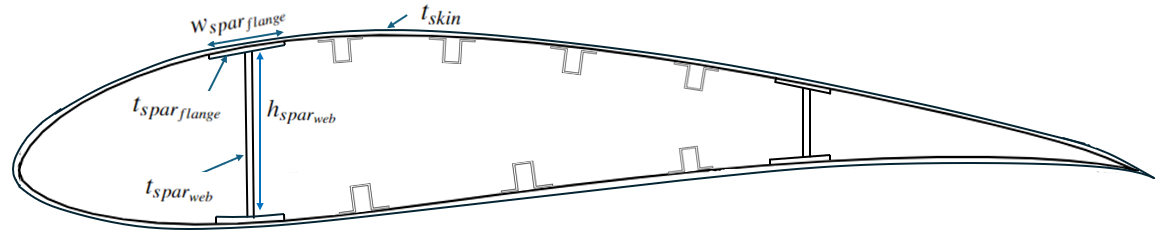
\includegraphics[width=0.8\linewidth]{figures/Structures/WingBoxStructure.png}
    \caption{Wing Box structure with optimisation parameters}
    \label{fig:wingboxexe}
\end{figure}

\begin{table}[H]
    \centering
    \caption{Wing structure parameters. The x locations [m] indicate the distance from the root in meters.}
    \label{tab:finalwingstructure}
    \sisetup{table-auto-round}
    \begin{tabular}{
        S[table-format=1.2]|
        S[table-format=3.0]
        S[table-format=1.2]
        S[table-format=1.1]
        S[table-format=1.1]
        S[table-format=1.0]
        S[table-format=1.0]
    }
        \toprule
         $x$ [\unit{m}] & $h_{\text{spar}_\text{web}}$ [\unit{mm}] & $t_{\text{spar}_\text{web}}$ [\unit{mm}] &  $t_{\text{spar}_\text{flange}}$ [\unit{mm}] & $t_\text{skin}$ [\unit{mm}] & $N_{\text{stringers}_\text{top}}$ [\unit{-}] & $N_{\text{stringers}_\text{bottom}}$  [\unit{-}] \\ \midrule
        0 & 227 & 1.5     & 2.8 & 1.5 & 4 & 3 \\
        0.85 & 211 & 1.5  & 2.8 & 1.5 & 4 & 3 \\
        1.8 & 192 & 1.34  & 2.5 & 1 & 4 & 3 \\
        2.15 & 185 & 1.31 & 2.5 & 1 & 4 & 2 \\
        4.5 & 140 & 1.11  & 2.5 & 1 & 3 & 2 \\
        6.84 & 94 & 0.91  & 2.5 & 1 & 2 & 1 \\ \bottomrule
    \end{tabular}
    \label{tab:finalwingstructure_transposed}
\end{table}

After the basic structure of the wing was designed, an STO folding wing type was chosen, inspired by the Grumman F4F-4 Wildcat.
The loads on the hinge were then used to size the titanium rod.
This resulted in a \qty{7.8}{\centi\m} radius and a mass of \qty{21.5}{\kg}.
An electrical linear actuator was finally chosen to allow for the hinge rotation.

\subsection*{\textit{Stability and Control}}
The report provides an in-depth analysis of the aircraft’s stability and control mechanisms, including the design of control surfaces and the empennage.
First and foremost, the design was analysed for controllability in the hover phase, making use of the ACAI algorithm \cite{du2015controllability}.
Based on the algorithm, the required centre-of-gravity (CG) range of the design between cruise and hovering has been computed.
Thus, a centre of gravity location of $X_{\text{CG}_{\text{cruise}}}=\qty{2.37}{\m}$ during cruise was established,
whereas in hover, the CG location was established to have a value of $X_{\text{CG}_{\text{hover}}}=\qty{3.68}{m}$.

Based on the CG ranges,
stability and controllability analysis can be performed during cruise to size the horizontal and vertical stabilisers.
Due to the ground footprint requirement, it was determined that a conventional vertical stabiliser is unfeasible.
Thus, an inverted V-tail concept was chosen for further design iterations.
Scissor plot analysis, as well as weathercock stability and engine inoperative controllability analysis, were performed to size the empennage.
The final empennage parameters are provided below:

\begin{table}[H]
    \begin{minipage}{0.49\textwidth}
        \centering
        
\includegraphics[width=0.65\linewidth]{figures/EO/img}
        \captionof{figure}{CG position during vertical and cruise flight}
        \label{fig:CGposition}
    \end{minipage}
    \begin{minipage}{0.49\textwidth}
        \centering
    \caption{Final Tail Design}
    \label{Final Tail Design}
    \begin{tabular}{
        @{}
            >{$}l<{$}
        |S[table-format=2.2]
            >{\collectcell\unit}l<{\endcollectcell}
        @{}
    }
        \toprule
        S_\text{h}               &  4.48         & m^2           \\
        S_\text{v}               & 2.73         & m^2            \\
        S_\text{tail}       & 7.21         & m^2            \\
        A_\text{v}             & 1.52         &    -           \\
        A_\text{h}              & 2.50         &    -           \\
        \Lambda_\text{h}   & 0.40         &          -     \\
        \Lambda_\text{v}  & 0.40         &            -   \\
        \nu         & 31.36         &       -    \\
        b_\text{tail}           & 4.59         & m              \\
        c_\text{r}               & 2.24         & m              \\
        c_\text{t}             & 0.90         & m              \\
        \bottomrule
    \end{tabular}
    \end{minipage}
\end{table}

Lastly, the ailerons were sized in order to provide roll control.
However, due to the increased roll moment caused by the battery placement, the ailerons were assumed to be placed throughout the entire wing.
This was still insufficient to provide the required roll control stated in the requirements, only achieving a value of \qty{60}{\degree} in \qty{6}{\s}, compared to the requirement of \qty{60}{\degree} in \qty{3.4}{\s}~\cite{roll_requirement}.


\subsection*{\textit{Autonomous Systems}}
The conceptual design of the autonomous system was discussed in this report.
To perform the route planning for the UAM, a multi-agent simple Probabilistic RoadMaps algorithm was selected \cite{PRM,todays_traveling_salesman}.

Furthermore, to facilitate unmanned guidance, three main control modes were deducted from the vehicle’s mission profile.
A position-tracking hexacopter control architecture with proportional derivative controllers was selected for vertical take-off, landing and hovering \cite{quadcopter_control_allocation}.
A gain-scheduling controller, with attitude
altitude and torque impedance controllers, controls the transition \cite{transition_control}.
Ultimately, the fixed-wing configuration is steered by a Model Predictive Contouring optimal controller \cite{MPC_justification,MPCC}.

Finally, a revised sensor selection was performed to ensure that all the required states can be measured directly or indirectly.
The obstacle detection and recognition are done by structured light stereo cameras and radar systems \cite{structured_light}.
This computer vision performs adequately in low light intensity and bad weather conditions.
The full state estimation of the UAM is done by GSNN GPS, IMU, pitot tube and thermal sensors.
Furthermore, motor speed encoders, voltmeters, and ammeters are chosen to regulate the inputs of the actuators.

\subsection*{\textit{Electric Power System}}
Knowing the total energy and maximum power required for the mission profile makes it possible to size the power system.
Firstly, a general literature study on lithium-ion batteries has been conducted.
From this, the discharge behaviour during the mission profile has been retrieved.
In particular, it has been made sure that the battery provides the necessary power at each flight phase.
This is done by having six battery packs, each containing 768 cells.
After knowing these parameters, it was possible to design the battery layout, and the cylindrical cells were chosen to build each pack.
Next, the battery degradation process was studied, the life cycle of the battery pack was estimated, and the charging power rating was given.
Lastly, battery cooling has been discussed, and liquid cooling has been chosen as a way to dissipate the heat during flight. The final parameters for the Electrical subsystem can be found in \Cref{tab_exe:FinalEPSValues}
\begin{table}[H]
\caption{Final electrical system Values}
\label{tab_exe:FinalEPSValues}
\centering
\begin{tabular}{cccccc}
    \toprule
$P_{\max}$ [kW] & $E_{\text{tot}}$ [kWh] & $U_{\text{nom}}$ [V] & $N_{\text{pack}}$ [-] & $N_{\text{cells}}$ [-] & $w_{\text{eps}}$ [kg]  \\\midrule
    343   & 120              & 710       & 6        & 768       & 400  \\
    \bottomrule
\end{tabular}
\end{table}



\section*{Resource Allocation and Financial Analysis}
The report outlines the resource allocation plan, detailing the interfaces between different subsystems and the overall project timeline.
A comprehensive financial analysis is provided,
including a detailed cost breakdown and an assessment of operational costs.
The analysis is conducted taking into account the production of 200 eVTOLs in the span of five years,
reaching the break-even point after 66 vehicles.
The production costs of the \textit{Swing} eVTOL are €1.42 million per unit, while the direct operational costs are €0.53 million per year, leading to €181 per flight hour. This breakdown does not, however, include the profit margins of the operator, thus making the cost to the final customer higher. Lastly, financial analysis has shown a return on investment of 10\%, making the \textit{Swing} eVTOL captivating for potential investors.

% This section ensures the project's economic feasibility and highlights the potential for a strong return on investment.



\section*{Production Plan}
The production plan covers the entire manufacturing process, from the early stages of part design to the final assembly. Firstly, some considerations have been made about vertical and horizontal integration methods of the production process, analysing advantages, disadvantages, and competitors' choices. From this analysis, based on various criteria such as costs or supply chain, it has been possible to decide whether to produce each subsystem in-house or outsource the production. This resulted in most of the components being outsourced while producing in-house novel technologies that are highly specific to the project. Lastly, the production line configuration has been explored, deciding to follow the commercial aeroplane manufacturers’ model, dividing the process into several stations for the different subsystems.

\section*{Sustainability Approach}
A key focus of the project is sustainability.
The report emphasises the eVTOL's energy consumption via missions analysis (\Cref{tab:energymissionsexe}) and its potential in revolutionising UAM. Emissions are evaluated, with low emissions predicted thanks to the low cruise speed of 200km/h.
A \enquote*{cradle-to-cradle} approach is adopted to minimise environmental impact, ensuring the repurposing of most of the vehicle components which are not directly recyclable. The impact of the \textit{Swing} on urban environments is then evaluated, with a forecasted drastic alleviation of traffic congestion and significant improvements in urban noise and air pollution. Finally, economic potential is also predicted with the introduction of this vehicle. This is thanks to the creation of new job opportunities, enhanced connectivity between cities, and a boost in tourism.


\begin{table}[H]
\caption{Sample missions energy consumption. Vertical flights include take-off and landing hovering phases.}
\centering
\begin{tabular}{l|c|c|c|c|c}
\textbf{} & \textbf{D$_\text{ground}$[km]}  & \textbf{D$_\text{air}$ [km]}  & \textbf{Avg EV [kWh]}  & \textbf{Joby s4 [kWh]} & \textbf{Swing [kWh]}  \\ \toprule
LCY-LHR & 62  & 35  & 12 & 90 & 33    \\
AMS-BRU  & 203 & 158 & 38 & 128 & 53   \\ \bottomrule
\end{tabular}
\label{tab:energymissionsexe}
\end{table}

\section*{Final Design Overview}
The final design can be found in \Cref{fig_exe:design_inhover,fig_exe:design_incruise}. The final parameters of the \textit{Swing eVTOL} can be found in \Cref{tab:execond_param}.

\begin{table}[H]
\centering
\caption{Final design parameters of the \textit{Swing eVTOL.}}
\label{tab:execond_param}
    \sisetup{table-format=4, parse-numbers=false, input-decimal-markers=x}
    \begin{tabular}{
        l
        S
        >{\collectcell\unit}l<{\endcollectcell}
        |l
        S
        >{\collectcell\unit}l<{\endcollectcell}
    }
    \toprule
    MTOW          & 1640 & kg   & Wing span       &   14.0  & m   \\
    OEM           & 1240 & kg   & Wing area       &   14.0  & m^2 \\
    Range         &  250 & km   & MAC             &    1.06 & m   \\
    Payload       &  400 & kg   & Fuselage length &    8.0  & m   \\
    Battery mass  &  400 & kg   & No. Engines     &    6    & -   \\
    Cruise speed  &  200 & km/h & Battery energy  &    125  & kWh \\
    Stall speed   &  105 & km/h & No. Passengers  &    4    & -   \\
    Total Power   &  344 & kW   & Production Cost &    1.42    & M€  \\
    \bottomrule
    \end{tabular}
\end{table}

\begin{figure}[h]
  \centering
\begin{subfigure}[b]{0.49\textwidth}
    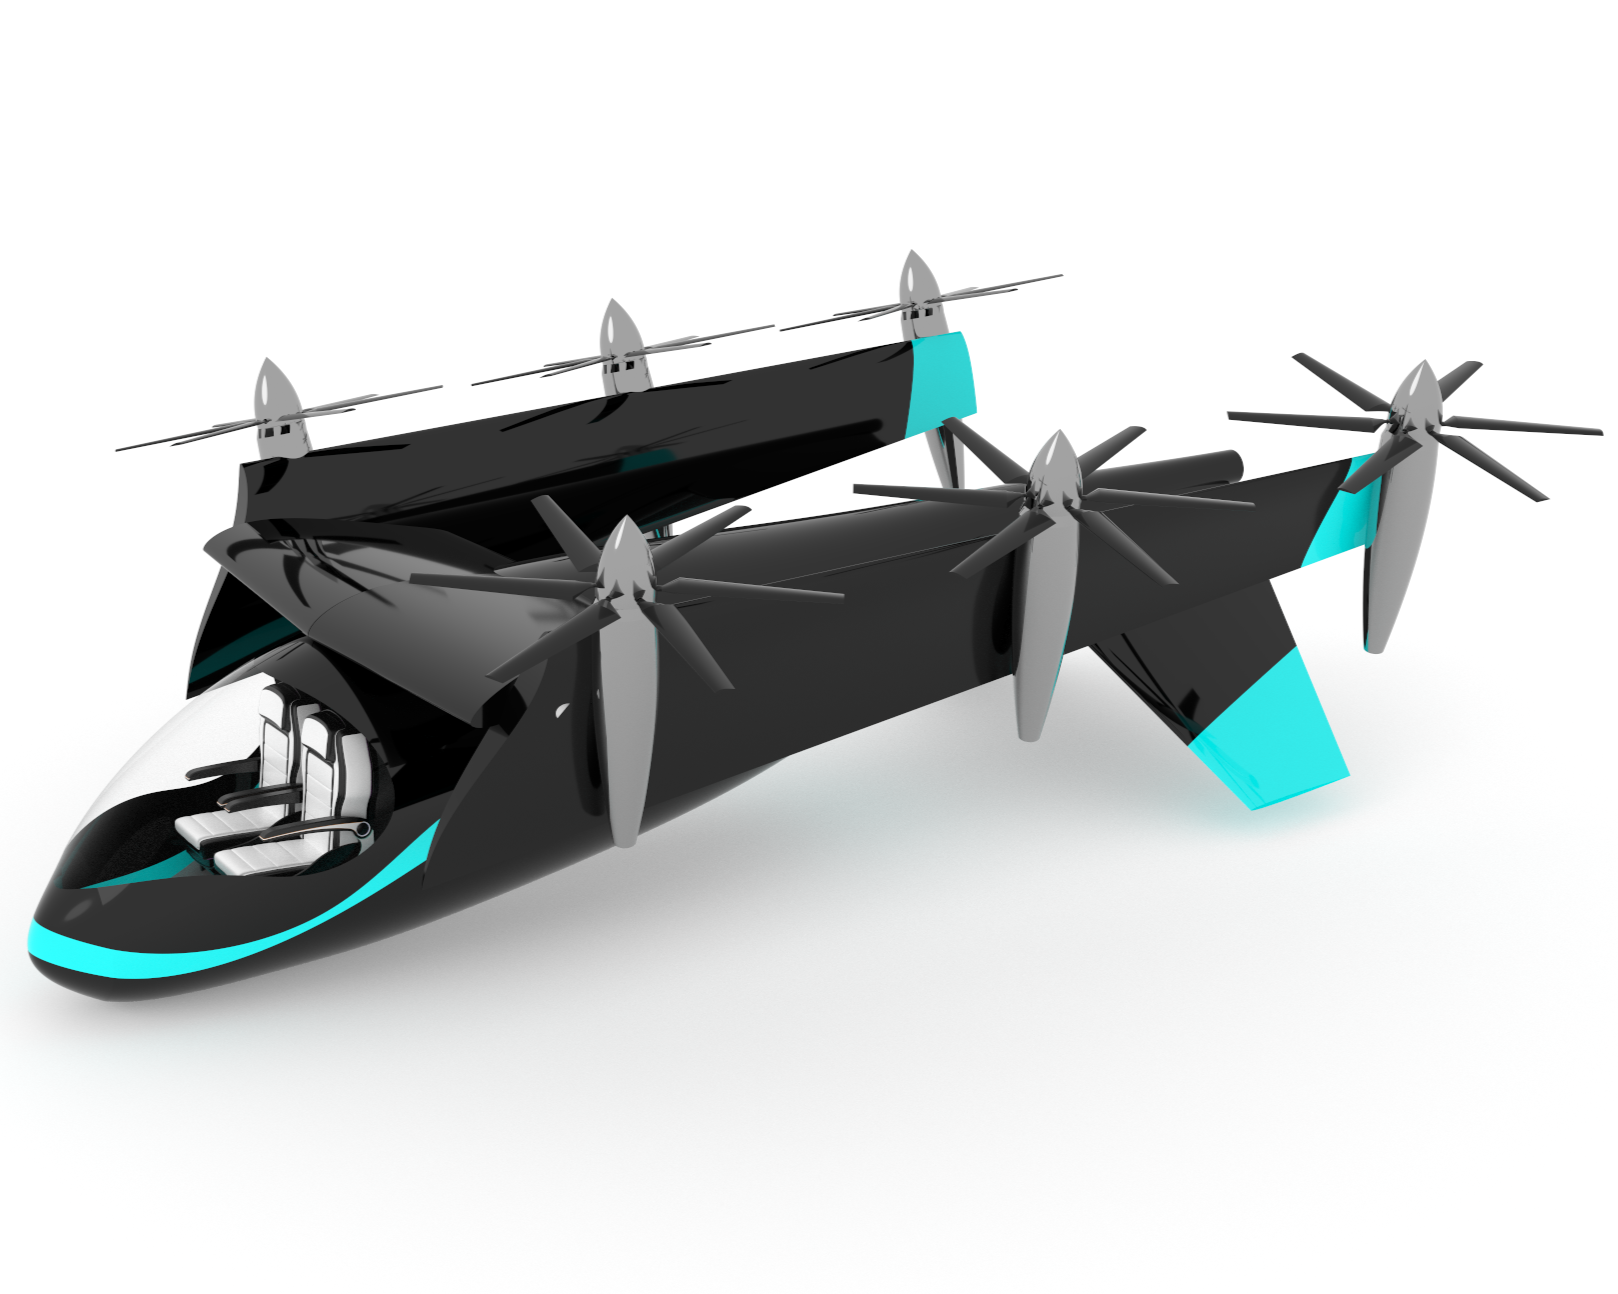
\includegraphics[width=1\linewidth]{Swing_eVTOL_ISO_hover.png}
    \caption{Final design of \textit{Swing eVTOL} in hover configuration}
    \label{fig_exe:design_inhover}
\end{subfigure}
\begin{subfigure}[b]{0.49\textwidth}
    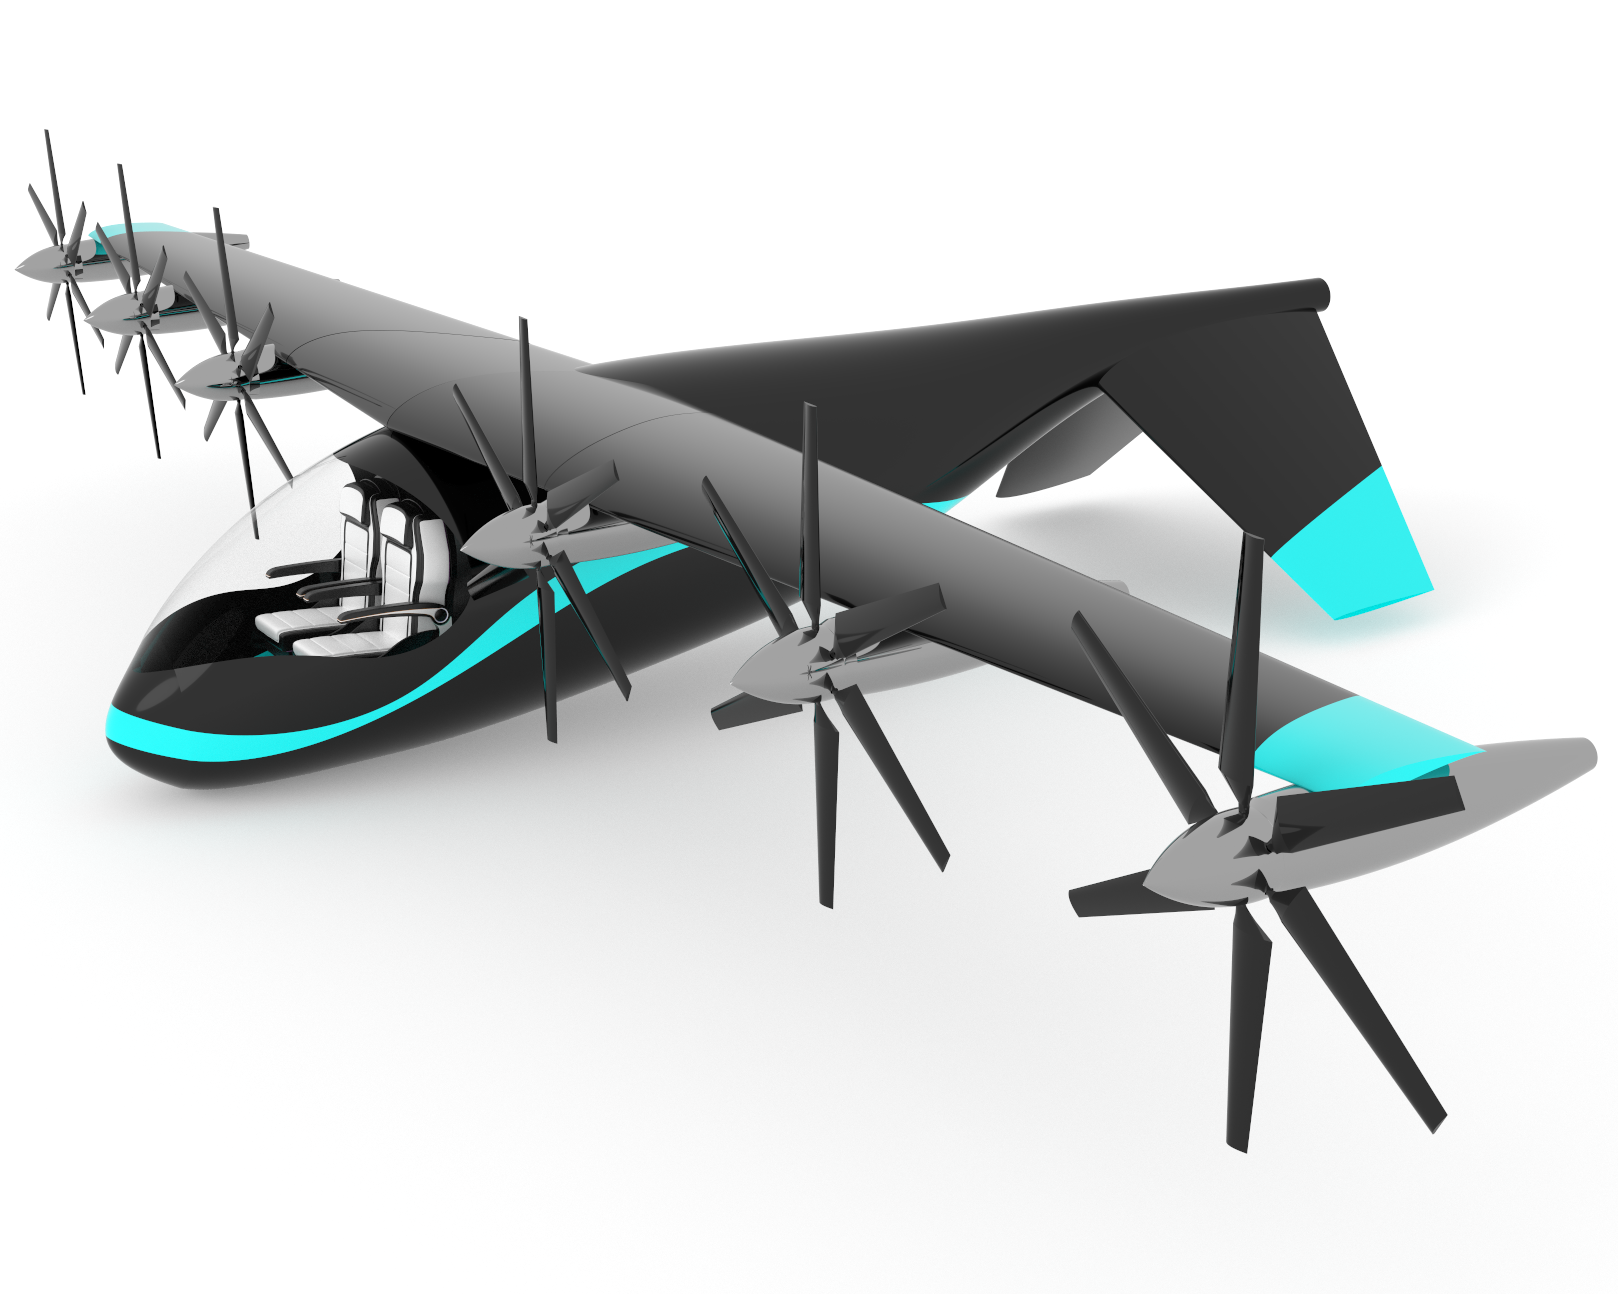
\includegraphics[width=1\linewidth]{Swing_eVTOL_ISO_cruise.png}
    \caption{Final design of \textit{Swing eVTOL} in cruise configuration}
    \label{fig_exe:design_incruise}
\end{subfigure}
\caption{Final design of \textit{Swing eVTOL}}
\label{fig_exe:Final_design_swing}
\end{figure}